\chap{Cardiovascular Physiology}
This chapter is intended to give a brief introduction to cardiovascular physiology and an overview of a few key anatomical and pathophysiological concepts, such as heart failure and pulmonary embolism, which will be necessary for the context of the continued discussion.

\sect{Circulation}
The purpose of the circulatory system is to transport the blood around the body. The blood supplies the metabolism of the cells and transports waste products such as carbon dioxide ($\textrm{CO}_2$) away from the cells~\cite{Hall2016}. The plumbing of this system consists of arteries and veins. In the tissues, the arteries and the veins meet in the capillary bed, where oxygen ($\textrm{O}_2$) is transported from red blood cells to tissue. At the center of this system is the heart, which under normal conditions, pumps blood at a given rate to meet the metabolic demands of all tissues. The veins from the systemic circulation eventually drain into the superior and inferior \emph{vena cava}, which enters the heart through the right atrium. The blood is then ejected into the pulmonary circulation through the \emph{truncus pulmonalis} or the main pulmonary artery, which bifurcates into the right pulmonary artery (RPA) \Nomenclature{RPA}{Right pulmonary artery} and the left pulmonary artery (LPA). \Nomenclature{LPA}{Left pulmonary artery} Note that in the pulmonary circulation, the roles of the arteries and the veins are reversed. The pulmonary arteries carry deoxygenated blood from the right side of the heart to the lungs to become oxygenated in the alveoli, where the blood releases $\textrm{CO}_2$ and absorbs $\textrm{O}_2$ through the process of diffusion. The pulmonary veins carry oxygenated blood back to the left side of the heart, where it is ejected back into the systemic circulation through the \emph{aorta}, see Figure~\ref{fig:circulation}.
\begin{figure}[htbp]
\centering
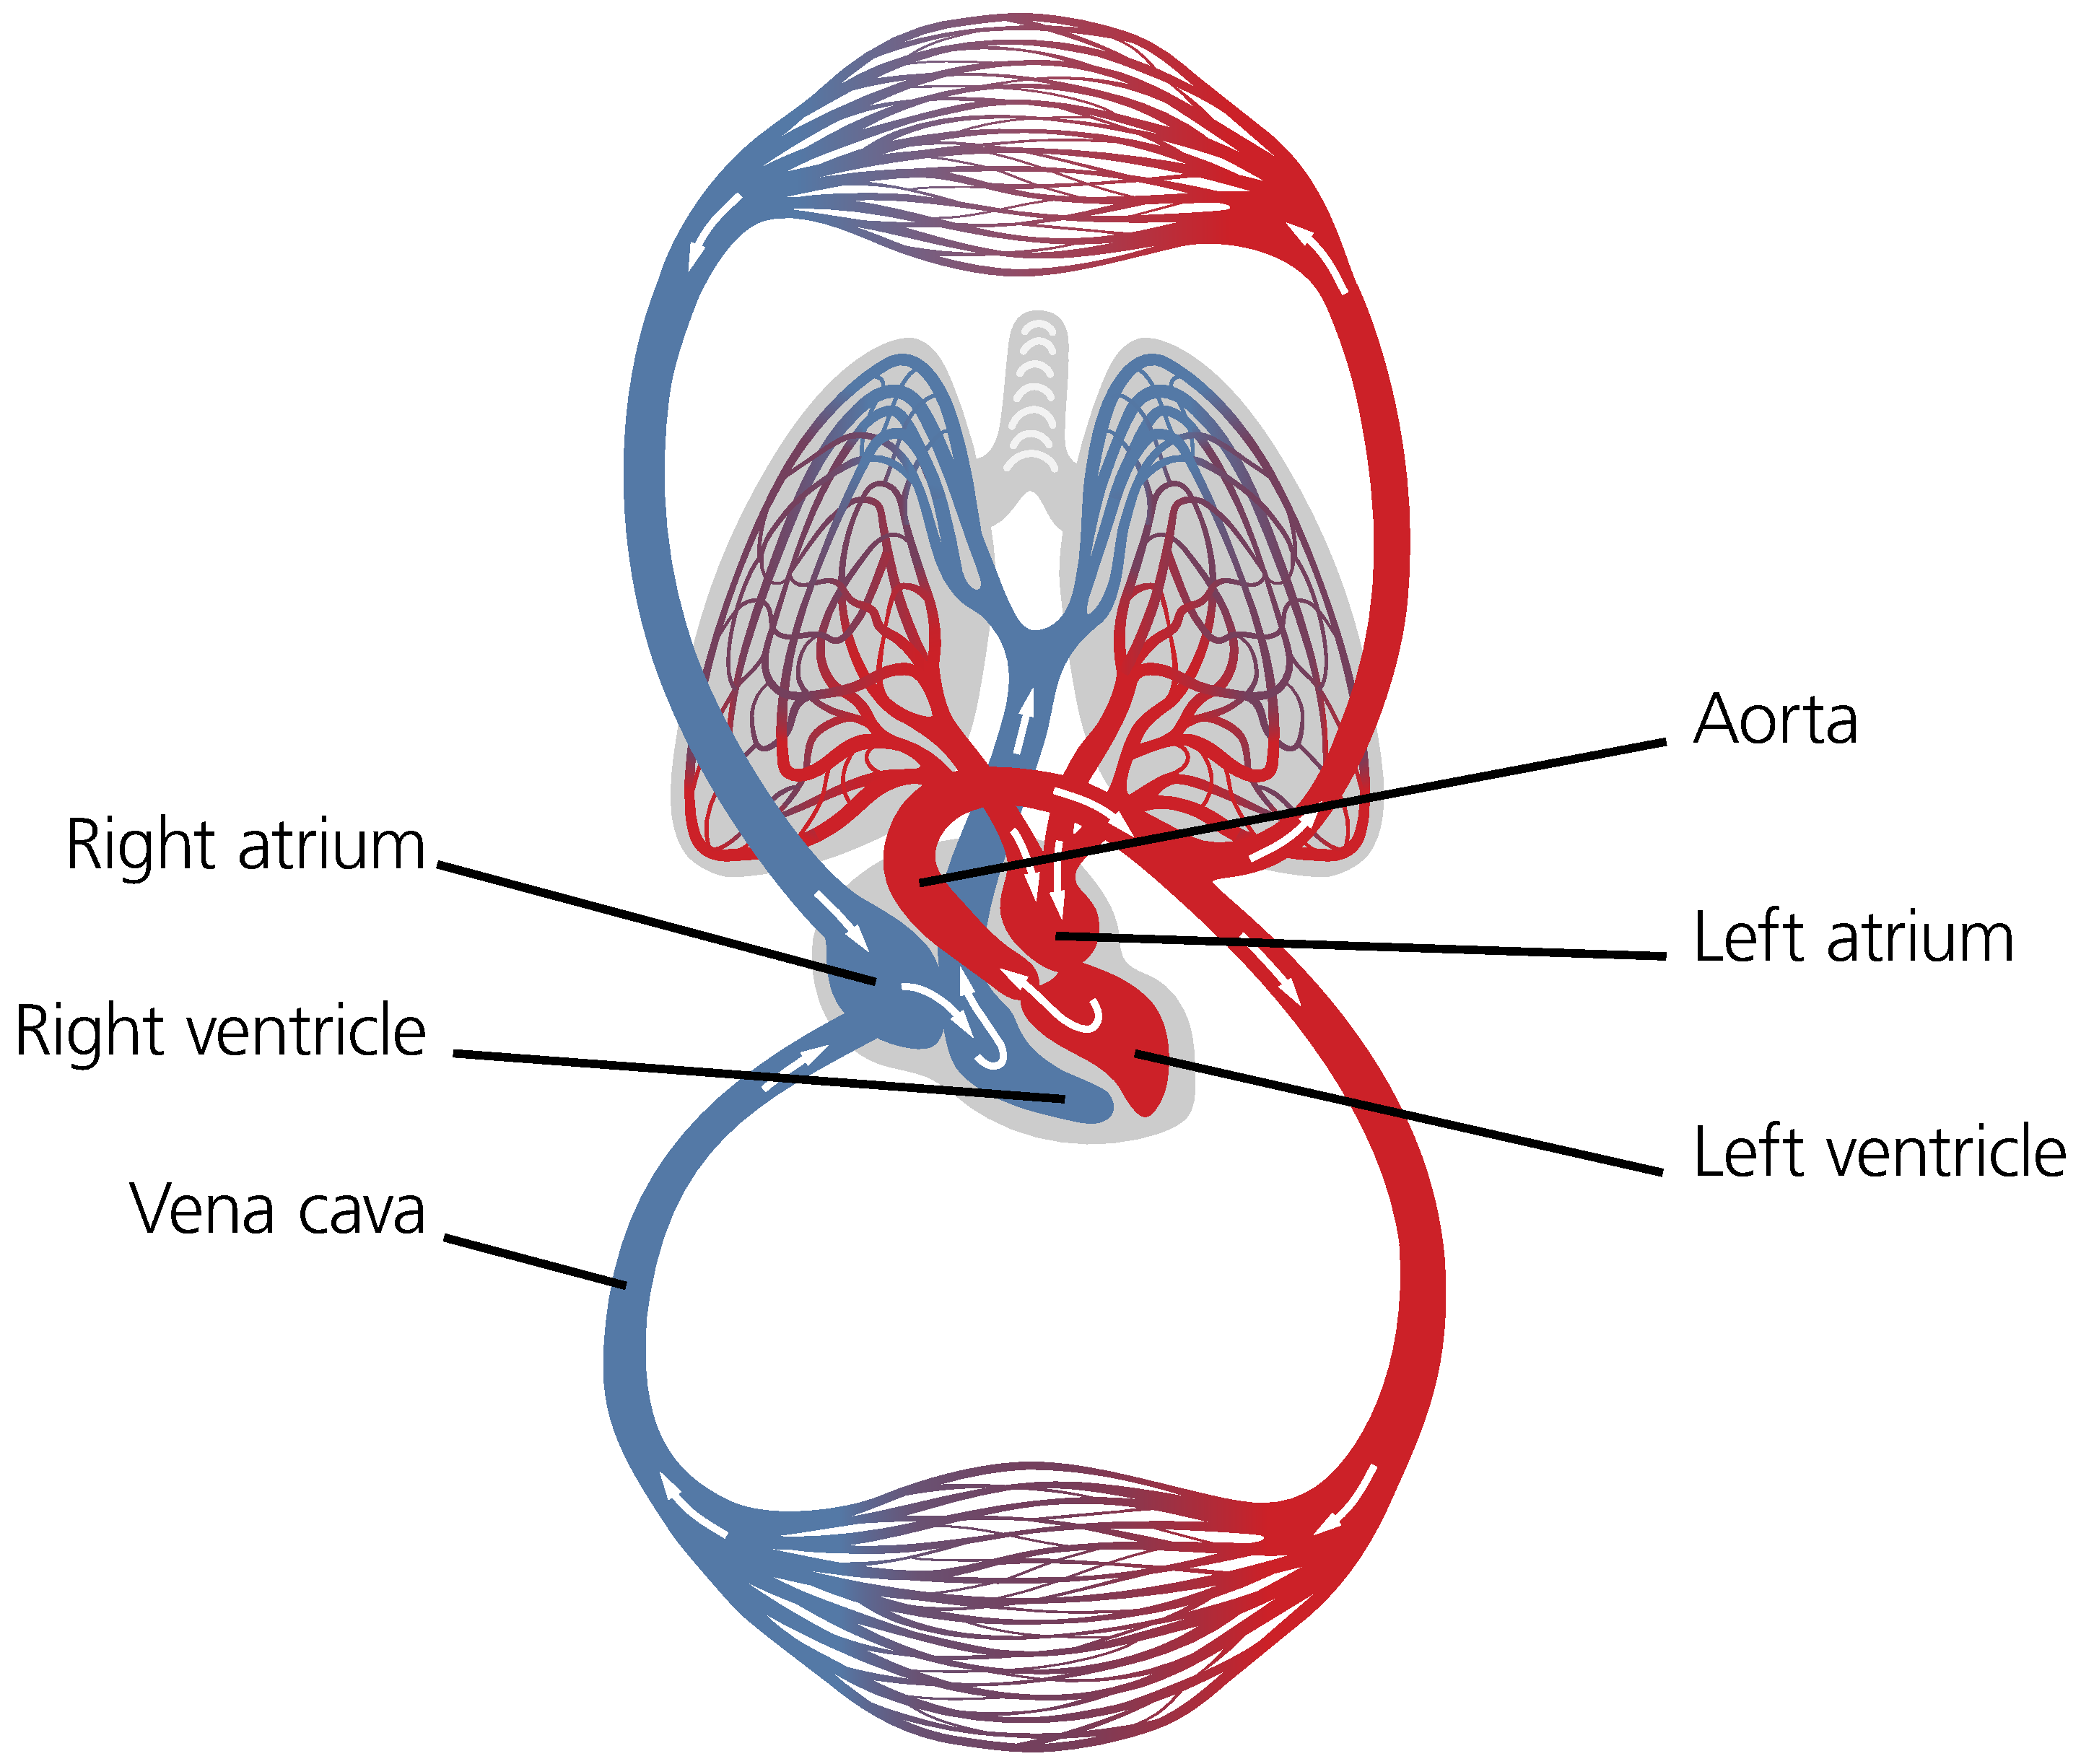
\includegraphics[width=0.75\textwidth]{circulation}
\caption{A schematic overview of the circulatory system. (Licensed under Adobe Stock Standard license)}
\label{fig:circulation}
\end{figure}

\sect{The heart}

\begin{figure}[htbp]
\centering
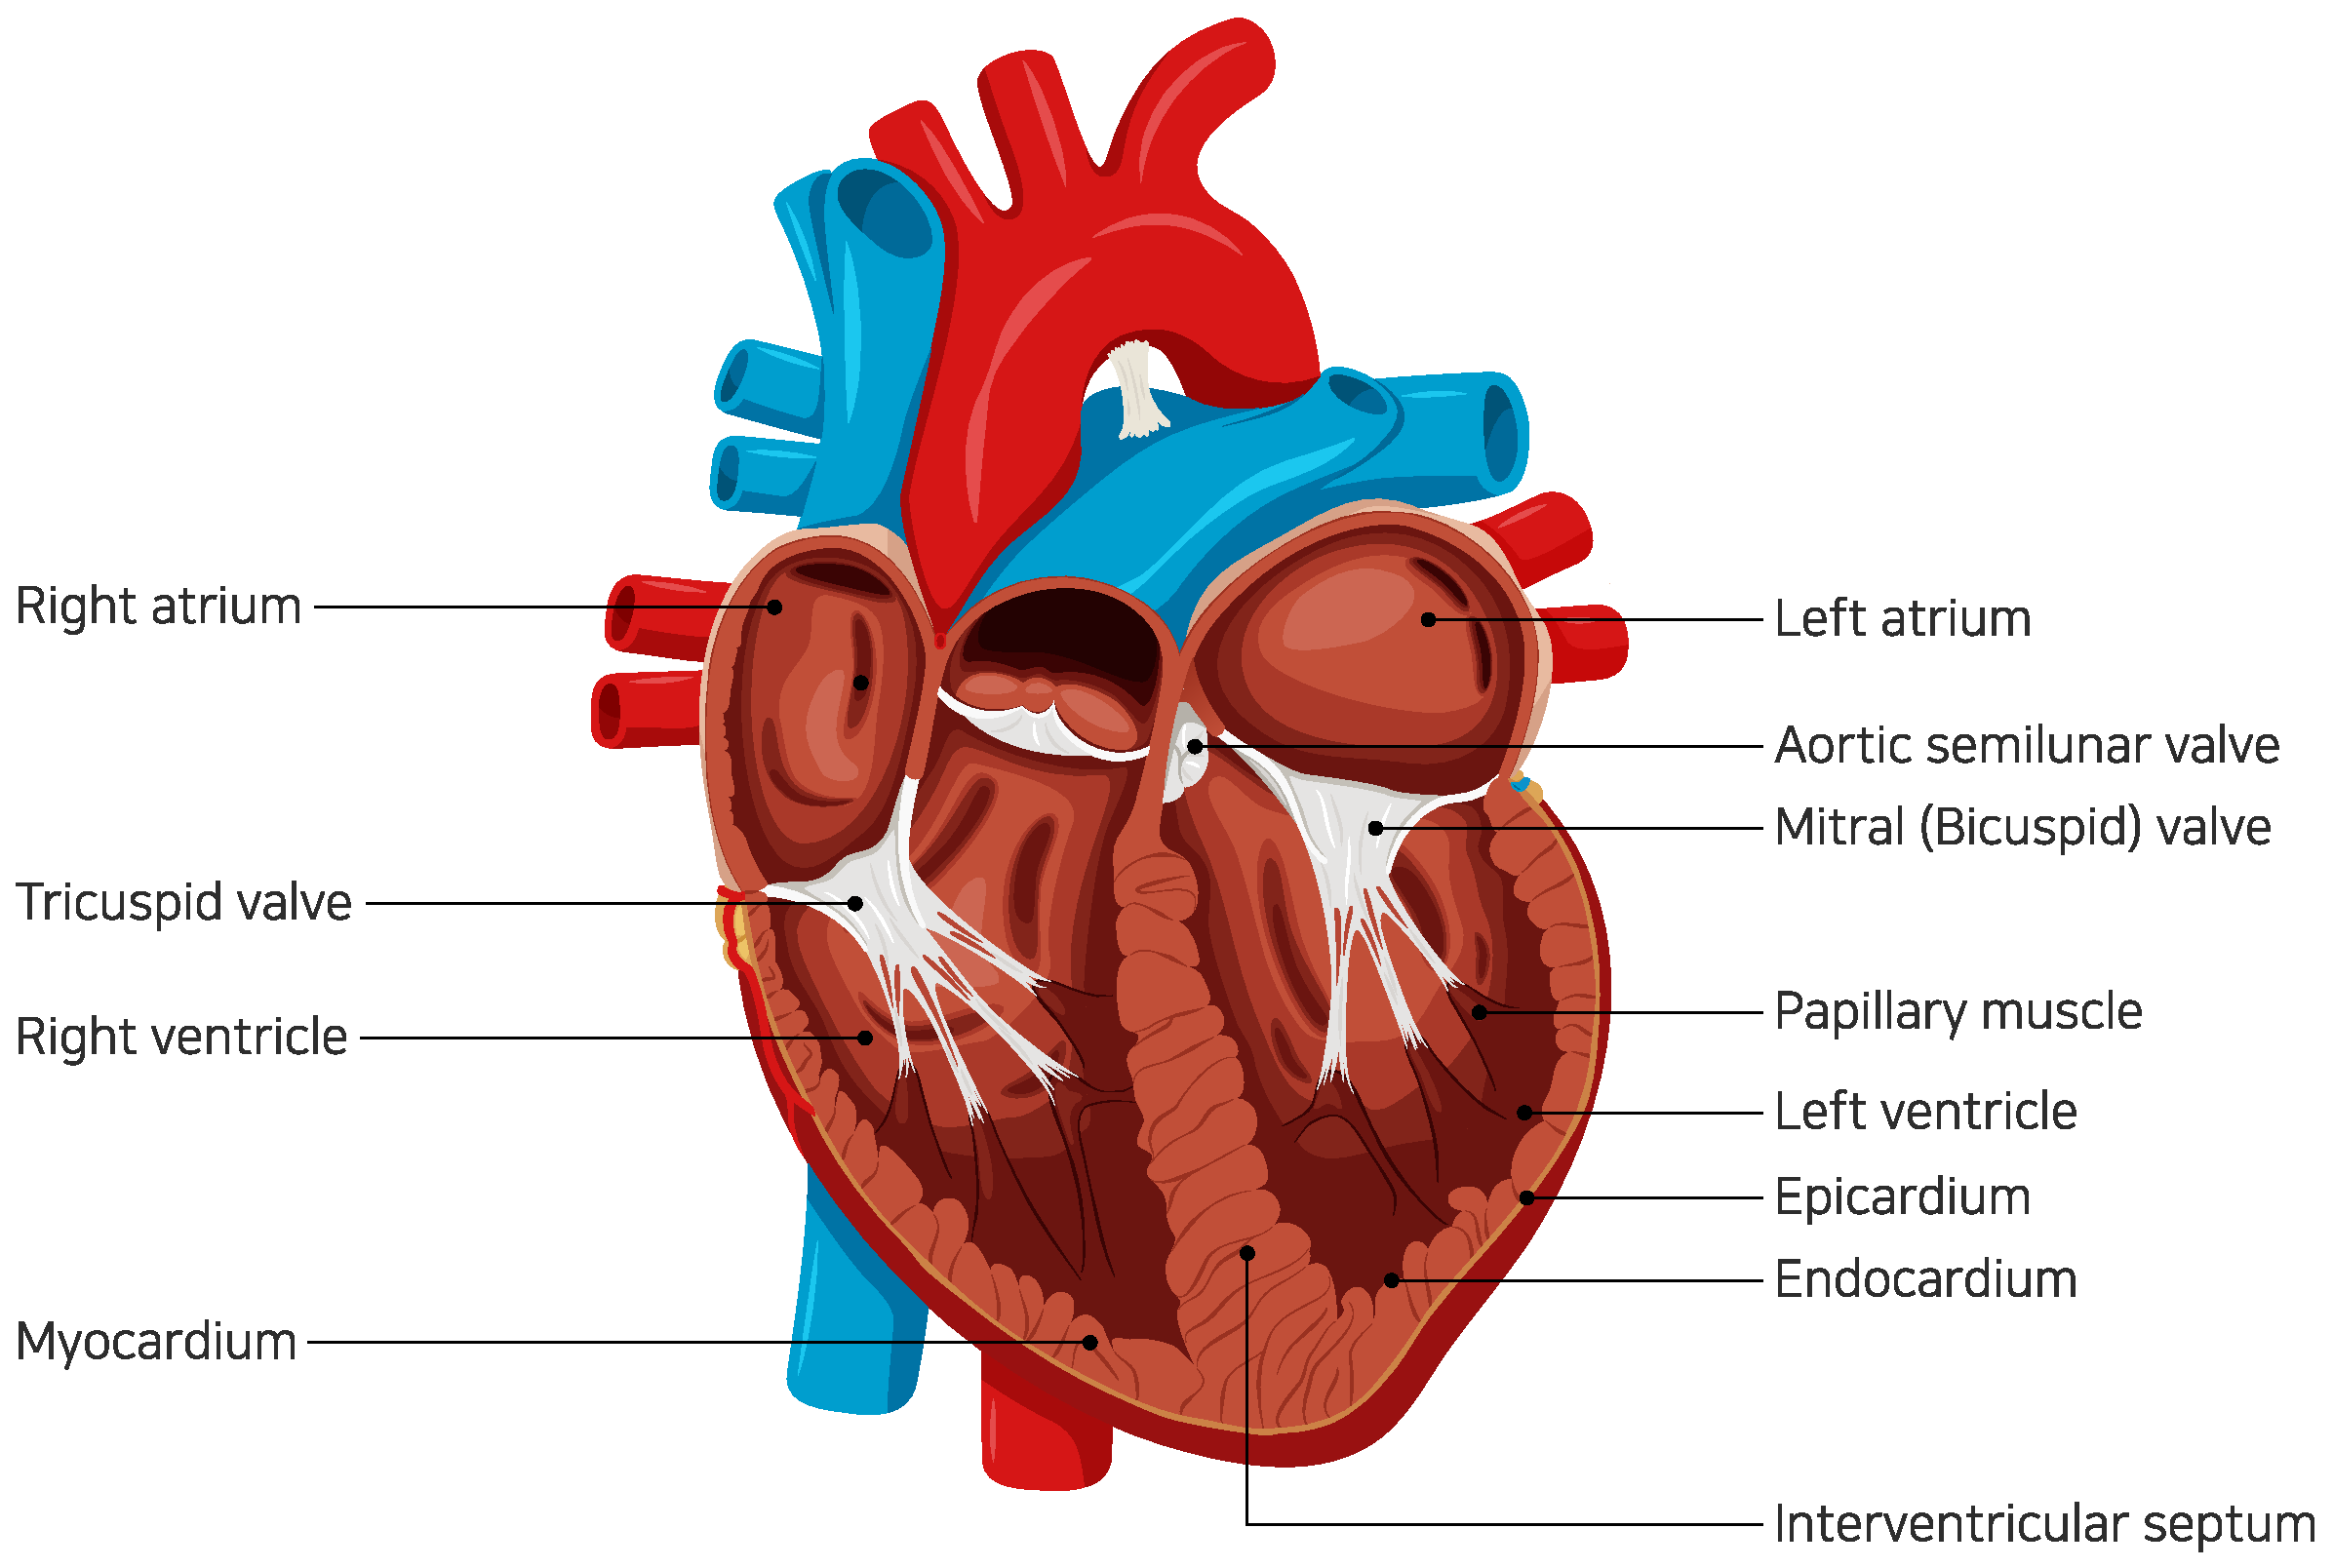
\includegraphics[width=0.75\textwidth]{heart}
\caption{A schematic overview of the human heart viewed from the front. (Licensed under Adobe Stock Standard license)}
\label{fig:heart}
\end{figure}
Both anatomically and functionally, the heart is divided into a left and a right side. Both sides have an atrium and a ventricle. The two ventricles are separated by the interventricular septum, see figure~\ref{fig:heart}.
\begin{figure}[tbp]
\centering
\includegraphics[width=0.75\textwidth]{valves}
\caption{A schematic overview of the valves of the heart viewed from above. (Licensed under Adobe Stock Standard license)}
\label{fig:valves}
\end{figure}
Venous blood is carried in the vena cava to the right side of the heart where it enters the right ventricle through the tricuspid valve, sometimes known as the right atrioventricular valve. From there, the blood is ejected through the pulmonary valve into the pulmonary circulation. Oxygenated blood then returns to the left atrium and enters the left ventricle through the mitral valve, sometimes known as the left atrioventricular valve. From the left ventricle, the blood then gets ejected back out into the systemic circulation through the aortic valve. 

\sect{Systolic function}
Systolic function refers to the heart's ability to pump forcefully enough to eject a sufficient amount of blood into the systemic circulation, to meet the oxygen and metabolic demand. The systolic function of the heart can be asserted by measuring a few key parameters, namely the end-diastolic volume (EDV)\Nomenclature{EDV}{End-diastolic Volume} and the end-systolic volume (ESV)\Nomenclature{ESV}{End-systolic Volume}. These measurements refer to the volume of blood in the left ventricle at the end of ventricular filling (end-diastole) and the end of ventricular contraction (end-systole), measured in ml. Using MRI, these measurements are acquired through manual and/or automatic segmentation of the left ventricle. From the ESV and the EDV, a few further parameters can be derived, namely the stroke volume (SV), \Nomenclature{SV}{Stroke volume} defined as $\textrm{SV} = \textrm{EDV} - \textrm{ESV}$, and the ejection fraction (EF), defined as \Nomenclature{EF}{Ejection fraction} $\textrm{EF} = \textrm{SV}/\textrm{EDV,}$ measured in percent.

\sect{Diastolic function}
Assessment of diastolic dysfunction using MRI remains challenging~\cite{Caudron2011}. Whereas some progress has been made in recent years~\cite{Flachskampf2015, Seemann2018}, the current non-invasive reference standard for assessing diastolic function is echocardiography~\cite{Nagueh2016}. The diagnosis encompasses both functional and structural parameters such as the peak in-flow velocity over the mitral valve during early filling (E) and late filling (A), and the peak velocity of the mitral annulus during early filling (e'). The E/A ratio is associated with the pressure gradient between the atrium and the ventricle, where an E/A ratio $>1$ is considered normal. The e' velocity reflects the velocity at which the myocardial muscle fibers lengthen in early diastole, and a reduced e' velocity may indicate diastolic dysfunction. The ratio $\textrm{E}/\textrm{e'}$ is also important as it is associated with the left ventricular filling pressure~\cite{Park2011}. See Figure~\ref{fig:echo} for an example of E, A and e' measurements using Doppler echocardiography. The remaining parameters used in echocardiographic assessment of diastolic dysfunction are the left atrial volume index (LAVI), \Nomenclature{LAVI}{Left atrial volume index} indexed to the body surface area (BSA),~\cite{Mosteller1987} \Nomenclature{BSA}{Body surface area} and the tricuspid regurgitant jet velocity. LAVI is an independent predictor of death and is associated with chronically elevated filling pressures~\cite{Pritchett2005}. The tricuspid regurgitant jet velocity, which through the simplified Bernoulli equation can be used to estimate the pressure gradient~\cite{Baumgartner2009}, which in turn can be related to pulmonary artery pressure as the sum of the pressure gradient and the right atrial pressure~\cite{Aduen2011}. Left atrial volume can easily be derived by CMR, and recent developments have suggested non-invasive measurements of pulmonary artery pressure derived by phase-contrast CMR~\cite{Reiter2013, Ramos2020}.
\begin{figure}[htbp]
\centering
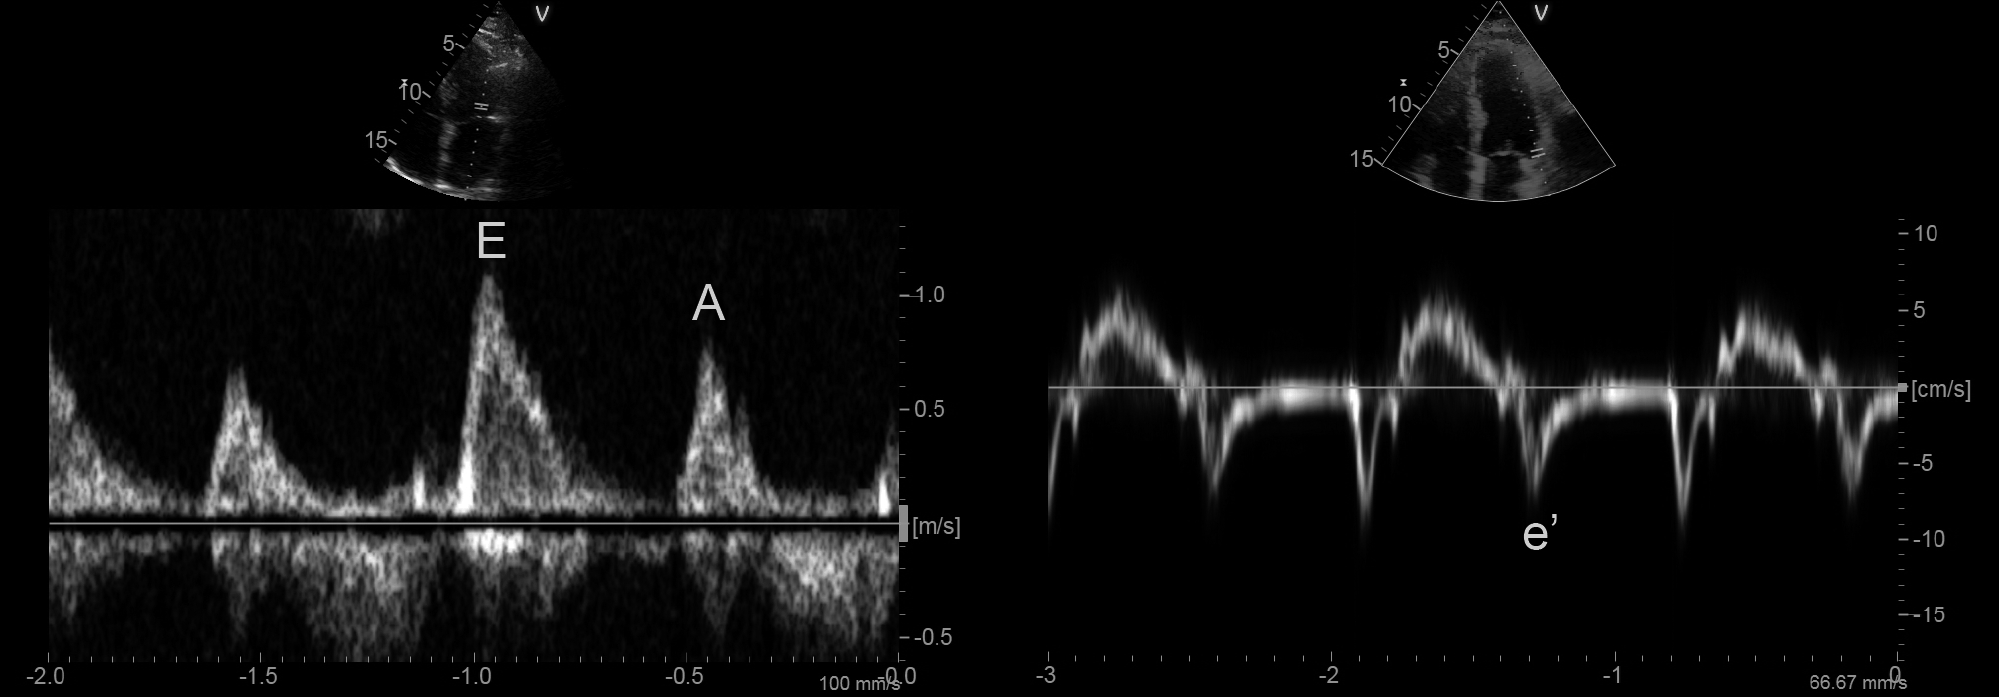
\includegraphics[width=\textwidth]{echo.png}
\caption{Example of key diastolic dysfunction parameters, such as trans-mitral inflow during early- and late filling (E \& A), and tissue velocity during early-filling (e') using Doppler echocardiography.}
\label{fig:echo}
\end{figure}
\sect{Heart failure}
Heart failure (HF)\Nomenclature{HF}{Heart failure} is defined as the condition when the heart cannot sufficiently pump blood to meet the oxygen demand under normal filling pressures~\cite{Hall2016}. Depending on the EF of the patient, heart failure can either be labeled heart failure with reduced ejection fraction, \Nomenclature{HFrEF}{Heart failure with reduced ejection fraction} or heart failure with preserved ejection fraction (HFpEF) \Nomenclature{HFpEF}{Heart failure with preserved ejection fraction}. Recent guidelines also specify a condition labeled heart failure with mid-range ejection fraction (HFmrEF) \Nomenclature{HFmrEF}{Heart failure with mid-range ejection fraction}\cite{Ponikowski2016}.

The cutoff values for the three types of heart failure are defined as
\begin{itemize}
    \item HFrEF: EF $<40\% $
    \item HFmrEF: $40\% \leq \textrm{EF} < 50\% $
    \item HFpEF: EF $\geq 50\% $
\end{itemize}
The pathophysiological mechanisms of HFpEF are somewhat contentious~\cite{Pfeffer2019}, yet most evidence points towards an impaired diastolic function~\cite{Nagueh2019}.

\sect{Pulmonary embolism}
Acute pulmonary embolism (PE) \Nomenclature{PE}{Pulmonary embolism} is a medical condition characterized by acute obstruction of the pulmonary arteries by a solid, liquid, or gaseous mass that originated somewhere else in the body. The most common cause is a thrombus formed in the deep veins, so-called deep vein thrombosis (DVT) \Nomenclature{DVT}{Deep vein thrombosis}~\cite{Goldhaber2012}. A thrombus can break loose and follow the veins back into the vena cava, where it may enter the right side of the heart and be ejected out into the arterial side of the pulmonary circulation, where it may cause a blockage of the blood flow as the vessels narrow. Whereas acute PE is a serious condition, the clinical presentation can be rather non-specific, with symptoms such as chest pain or shortness of breath~\cite{Hampson1995}. Therefore, imaging is an integral component in the diagnosis of pulmonary embolism~\cite{Bounameaux2010}. Typically, this is done with contrast-enhanced computed tomography angiography (CTA) \Nomenclature{CTA}{Computed tomography angiography}. There are many comorbidities for PE that may contraindicate CTA, thus making MRI an attractive alternative method for diagnosis of pulmonary embolism~\cite{Stein2011}. 
\begin{figure}[hbt]
\centering
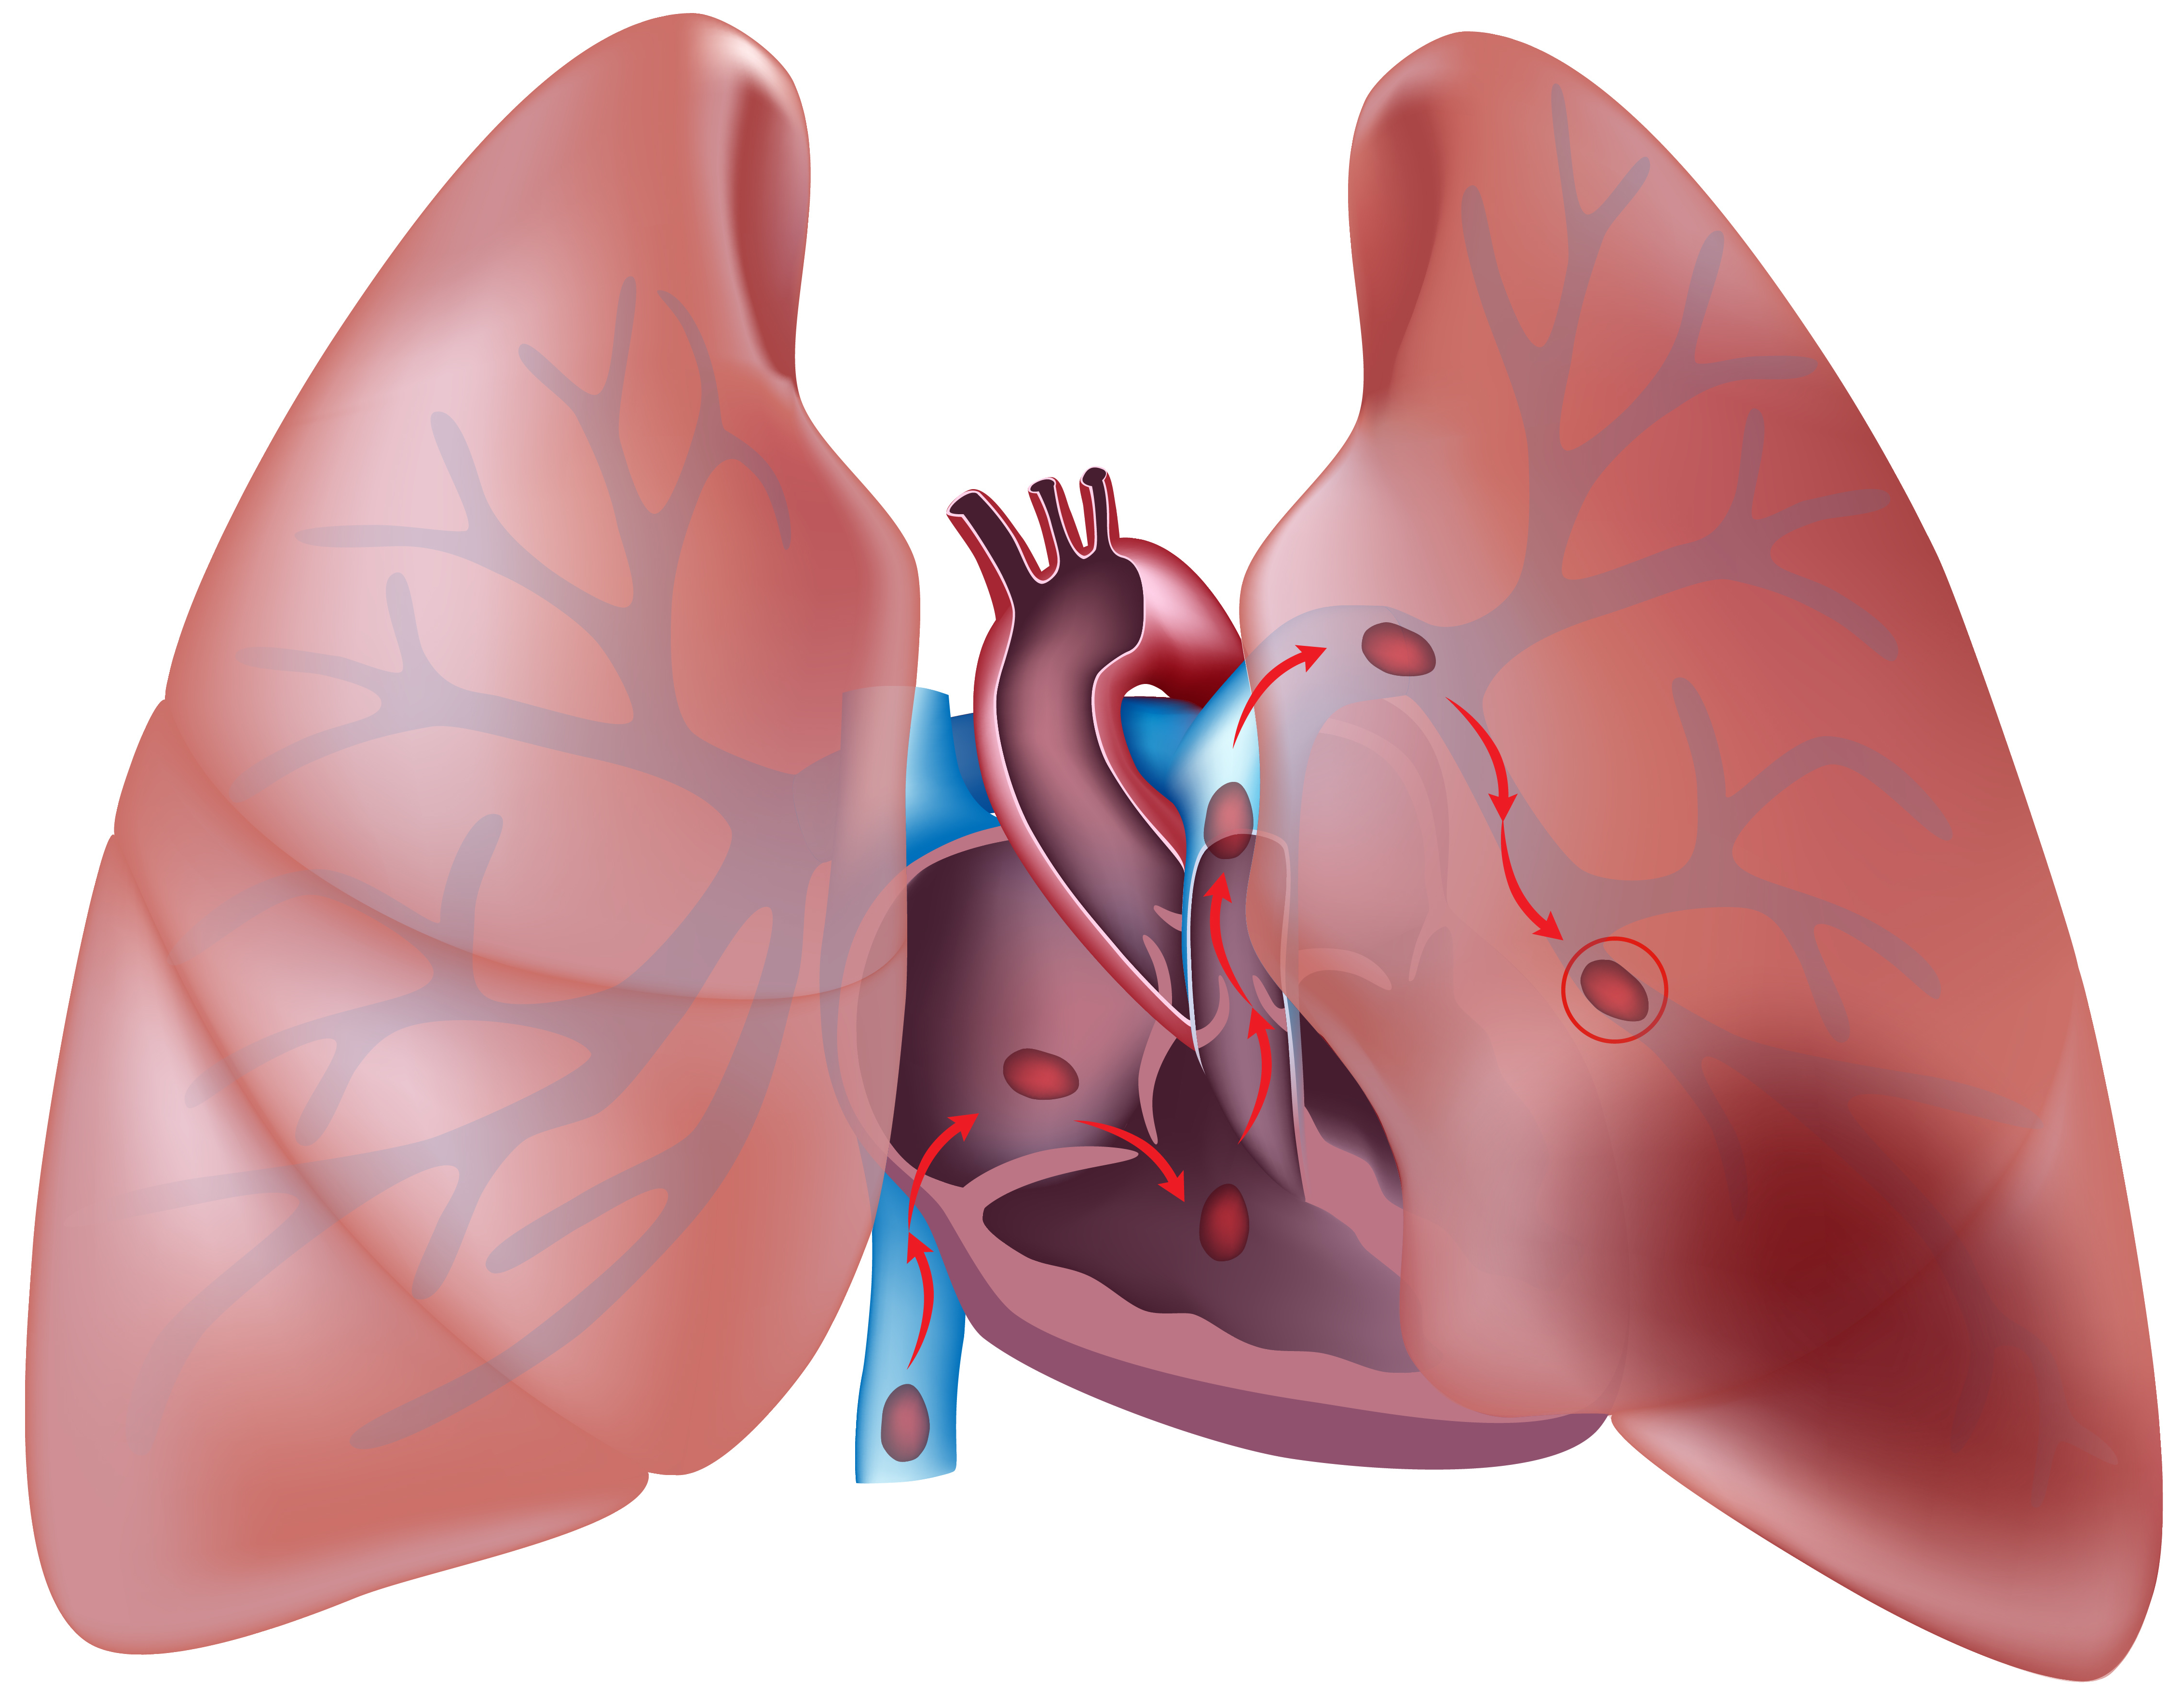
\includegraphics[width=\textwidth]{PE}
\caption{A schematic illustration of a thrombus originating in the deep veins entering the right side of the heart and ending up on the arterial side of the pulmonary circulation. (Licensed under Adobe Stock Standard license)}
\label{fig:pe}
\end{figure}
